
\subsection*{Graph Neural Networks} \label{sec:gn_layer}

GNNs are a class of neural networks working on sets of vertices and edges. Through different deep learning techniques such as convolution (Graph Convolutional Networks) \cite{kipf_semi-supervised_2017}, attention (Graph Attention Networks) \cite{velickovic_graph_2018} or recurrent layers (Graph Recurrent Networks) \cite{ruiz_gated_2020}, they exploit message passing mechanisms to learn the relations between neighboring nodes, and have shown great performances in many area of physics \cite{janny_eagle_2023, gladstone_gnn-based_2023, lam_graphcast_2023, garnier_meshmask_2024, lin_up-sampling-only_2024}.

Solving complex systems of partial differential equations, such as the Navier-Stokes equations, often requires mesh-based discretisation of the computational domain. These meshes are typically adapted to enhance numerical accuracy in critical regions while minimizing computational cost in less challenging areas \cite{coupez_solution_2013}. However, traditional deep-learning architectures, such as convolutional, recurrent, or fully connected layers, struggle to effectively handle the anisotropic and irregular nature of meshes. They either fail to capture local dependencies properly or do so at a prohibitive computational expense. Building on the founding that the deep-learning toolbox layers did not offer the possibility of learning arbitrary relations between elements of a set with relational structure such as a graph, Battaglia et al. \cite{battaglia_relational_2018} introduced the Graph Network (GN) layer, aiming to create a general framework for graph computation. Inspired from Message Passing Neural Networks \cite{gilmer_neural_2017} among others, this layer is designed to take a graph as input, process the graph with any subsequent model such as a neural network but not necessarily, and return a graph, using the nodes as entities with features, edges as relations between entities, and global attributes over the whole graph. 

We note an undirected graph $G = (V, E)$ with $V$ a set of vertices with $V = \{v_i\}_{i \in N^v}$ vertices attributes and $E$ a set of edges with $e_{ij}$ linking vertices with indexes $i, j$.

\begin{figure}[!ht]
    \centering
    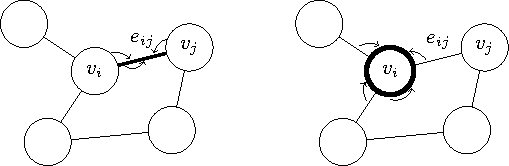
\includegraphics[width=0.6\textwidth]{figs/message_passing.pdf}
    \caption{Graph network updating edges (left) and nodes (right)}
    \label{fig:GN_updates}
\end{figure}

The GN updates edges attributes with an edge-update function $\varphi_E$, gathers a vertex neighborhood information by aggregating the updated edges connected to it with an aggregation function $\rho$, and updates the vertex with a vertex-update function $\varphi_V$ (\autoref{fig:GN_updates}). Because the update functions are shared over every nodes and edges, graph networks are adapted to learn local physical behavior over every relation in the graph. We purposefully left out global graph attributes here to avoid unnecessary complications of the framework, as we will not be using them.

\begin{align} \label{eq:GN}
    \tilde{e}_{ij} &= \varphi_E(e_{ij}, v_i, v_j) \nonumber\\
    \tilde{e}_i &= \rho(\{ \tilde{e}_{ij} \}_j) \\
    \tilde{v}_i &= \varphi_V(v_i, \tilde{e}_i) \nonumber
\end{align}

with $\tilde{e_{ij}}$ being the updated edge attributes from the initial edge attributes and the connected vertices attributes, $\tilde{e}_i$ being the aggregated information of all edges linked to vertex $i$, and $\tilde{v}_i$ being the updated vertex attributes from the initial vertex attributes and the aggregated neighborhood information.


\subsection{MeshGraphNet}
\label{sec:MGN}

Numerical physics simulations like CFD relies on meshes. Pfaff et al. \cite{pfaff_learning_2021} took advantage of this data structure and built a GNN model using physical meshes as inputs, designed for next-step prediction in physical problems such as flow field prediction around a cylinder or a wing profile. With the mesh information at $t$ (and potentially $t-1$), the trained network can predict the physical fields at $t+1$. By inferring on its own predictions, the network can generate a whole simulation with only a few initial timesteps to infer from; the MeshGraphNet (MGN) model has achieved state of the art results, being able to predict the temporal evolution of these systems during significant time periods while remaining coherent with the physical simulations. The MGN model learns the system's forward dynamics with an encode-process-decode (EPD) architecture (\autoref{fig:epd}), using multilayer perceptrons (MLPs).

\paragraph{Encoder} The encoder extracts all input features for nodes and edges from the graph $G_t$, which is derived from the mesh at time $t$. These features include physical properties such as velocity, pressure or stress, as well as geometrical attributes like edge lengths and node positions. The node and edge features are respectively encoded into latent spaces by the encoder MLP's $\epsilon_V$ and $\epsilon_E$ into latent spaces of size $d_v$ and $d_e$ the embedding dimensions, as graph nodes $v_i$ and edges $e_{ij}$, to constitute the latent space graph $Q_t$.


\paragraph{Processor} The processor then performs rounds of message passing by applying $L$ several successive GN layers. For each round of message passing, each node of the graph sends messages to its neighbors, which consist of the encoded and processed node’s and edge’s feature information. As in the GN layer described in \autoref{sec:gn_layer}, the neighbors aggregate and process these messages to gain a collective understanding of their local neighborhood, to update their own feature representation. This allows them to incorporate the new information received from their neighbors and refine their own states. Each of these GN layers has update functions $\varphi_E$ and $\varphi_V$ respectively for edges and nodes, as described in \autoref{eq:GN}. These functions are MLPs as well, with different sets of parameters for each GN layer, and the edge aggregation function $\rho$ is an element-wise summation. Performing several consecutive rounds of message passing allows the GNN to infer the evolution of the graph with information circulating over the whole domain, and to return an updated latent space graph $Q_{t+1}$ with updated node and edge latent vectors $\tilde{v}_i$ and $\tilde{e}_{ij}$. 

\paragraph{Decoder} Finally, the decoder translates the processed node vectors contained in the latent space updated graph $Q_{t+1}$ with a final MLP $\delta_V$ to a physical update, which is added to the input mesh in order to get the next-step physical mesh $G_{t+1}$ with updated physical fields. 

\begin{figure}[!ht]
    \centering
    \resizebox{0.8\textwidth}{!}{% \documentclass[tikz, border=0mm]{standalone}
% \usepackage{tikz}
% \usepackage{pgfplots}
% \usepackage{graphicx} % For subfigs
% \usepackage{amssymb}


% \tikzset{every picture/.style={line width=0.75pt}}
% \begin{document}
\begin{tikzpicture}
% INPUT
\node[anchor=south west, inner sep=0, xshift=0, yshift=-12] (input) at (0, 0) {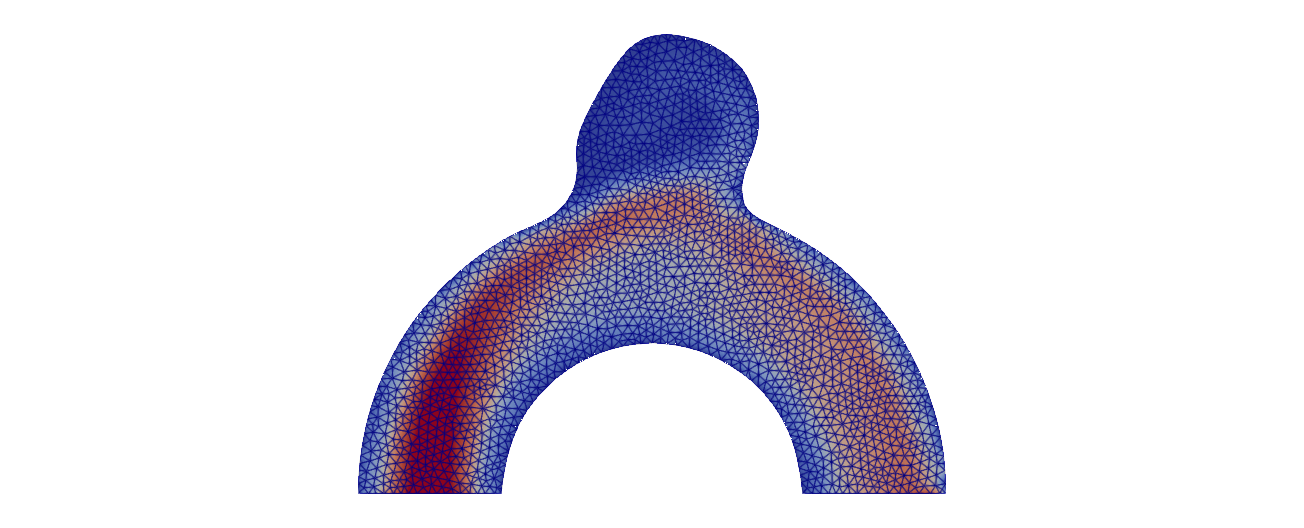
\includegraphics[trim={350 30 350 25}, clip, width=3cm]{tikz/figs/Anev_slice_moins.png}};

%OUTPUT
\node[anchor=west, inner sep=0, xshift=127, yshift=0] (output) at (input.east) {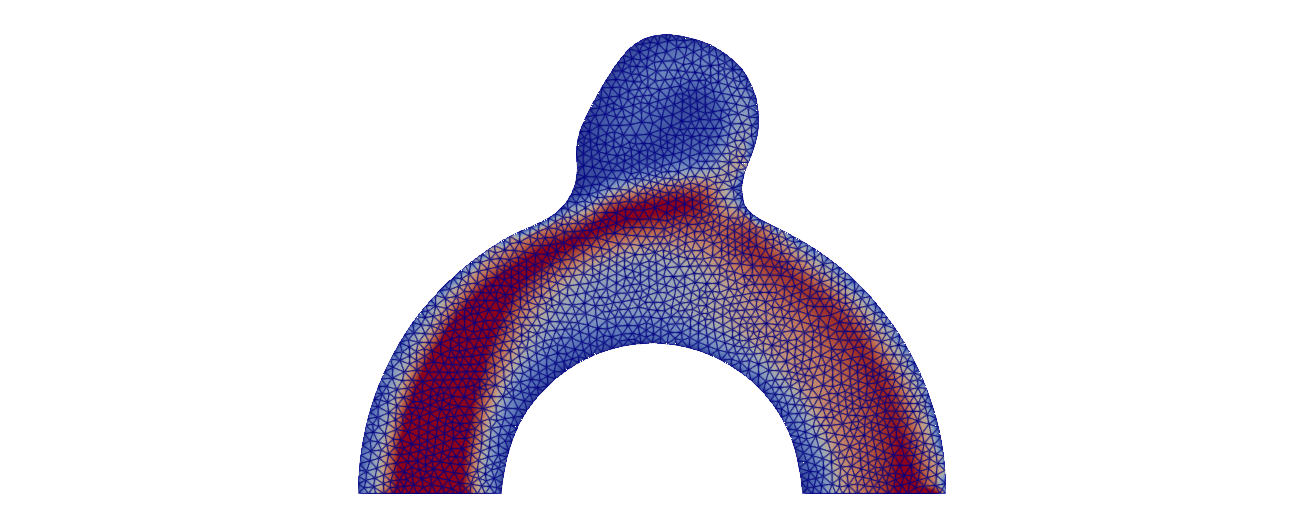
\includegraphics[trim={350 30 350 25}, clip, width=3cm]{tikz/figs/Anev_slice_plus.png}};

\node[circle, draw=black, inner sep=-1, anchor=east, xshift=-11.3
] (sum) at (output.west){+};

% ENCODER
\node[anchor=north, draw=black, inner sep=5, xshift=0, yshift=-30] (encoder) at (input.south) {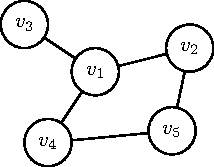
\includegraphics[width=2.0cm]{tikz/figs/graph.pdf}};

% PROCESSOR
\node[anchor=west, draw=black, thick, inner sep=0, xshift=21, yshift=5] (processor_1) at (encoder.east) {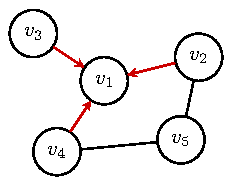
\includegraphics[width=2.2cm]{tikz/figs/processor.pdf}};

\node[anchor=west, draw=black, thick, inner sep=0, xshift=26, yshift=0] (processor) at (encoder.east) {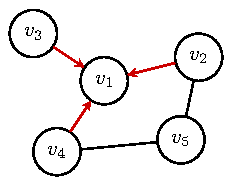
\includegraphics[width=2.2cm]{tikz/figs/processor.pdf}};

\node[anchor=west, draw=black, thick, inner sep=0, xshift=31, yshift=-5] (processor_2) at (encoder.east) {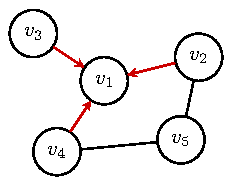
\includegraphics[width=2.2cm]{tikz/figs/processor.pdf}};


% DECODER
\node[anchor=west, draw=black, inner sep=5, xshift=26, yshift=0] (decoder) at (processor.east) {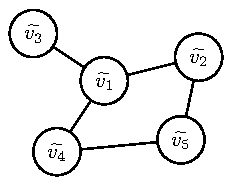
\includegraphics[width=2.0cm]{tikz/figs/decoder.pdf}};

% ARROWS
\draw[thick, shorten <= -15](input.south) edge[-stealth] node [left] {$U_t$} (encoder.north);
\draw[thick](encoder.east) edge[-stealth] node [above] {$Q_t$} ([xshift=-5]processor.west);
\draw[thick]([xshift=5]processor.east) edge[-stealth] node [above] {$Q_{t+1}$} (decoder.west);
\draw[thick]([xshift=-28]decoder.north) edge[-stealth] (sum.south);

\draw[thick, shorten <= -10](input.east) edge[-stealth] node [below] {$U_t$} (sum.west);
\draw[thick, shorten >= -10](sum.east) edge[-stealth] node [below, xshift=3] {$U_{t+1}$} (output.west);


% TEXTS
\node[anchor=south, inner sep=0, xshift=0, yshift=4] (text_input) at (input.north) {Input mesh $G_t$};
\node[anchor=south, inner sep=0, xshift=0, yshift=4] (text_output) at (output.north) {Output mesh $G_{t+1}$};
\node[anchor=north, inner sep=0, xshift=0, yshift=-4] (text_encoder) at (encoder.south) {Encoder};
\node[anchor=north, inner sep=0, xshift=0, yshift=-8] (text_processor) at (processor.south) {Processor};
\node[anchor=south, inner sep=0, xshift=0, yshift=8] (text_processor_2) at (processor.north) {\small $L$ rounds of processing};

\node[anchor=north, inner sep=0, xshift=0, yshift=-4] (text_decoder) at (decoder.south) {Decoder};
\node[anchor=south, inner sep=0, xshift=0, yshift=2] (text_sum) at (sum.north) {Graph update};


\node[anchor=south, inner sep=0, xshift=0, yshift=4] (blop_up) at (text_input.north) {};
\node[anchor=north, inner sep=0, yshift=-15, yshift=4] (blop_down) at (text_processor.south) { };

\end{tikzpicture}
% \end{document}
}
    \caption{Encode-process-decode (EPD) architecture \cite{pfaff_learning_2021} for velocity $U_{t+1}$ prediction from $U_t$.}
    \label{fig:epd}
\end{figure}

All the underlying processing and updating functions here are ReLU-activated 2 hidden-layer MPLs. The model learns the physical behavior by minimizing the differences between its predictions and the ground truth data computed with numerical solver, with a data loss being the mean square error, for a given physical quantity $a$:

\begin{equation} \label{eq:loss_data}
    \mathcal{L}_{data} = \underset{v \in V}{\mathrm{mean}} \ \vert \vert a_v - \tilde{a_v} \vert \vert^2_2
\end{equation}
with $a_v$ being the ground truth and $\tilde{a_v}$ the prediction at node $v$.

\subsection{Hemodynamics simulations} \label{sec:blood_flow}

The MeshGraphNet model has demonstrated excellent performance in predicting flow in 2D settings for benchmark fluid dynamics problems, such as incompressible steady flow around a cylinder and compressible flow around an airfoil. However, its ability to generalize to blood flow predictions in a three-dimensional environment remains an unexplored frontier and requires further investigation. The whole CFD problem setting for hemodynamics is described in details in \todo{ref to chapter:methods CFD}.

\todo{move WSS definition either methods or intro}
Several quantities of interest have been identified for risk assessment and treatment decision for unruptured intracranial aneurysms. Obtaining these quantities by post-processing the simulated velocity fields inside the aneurysm is of great interest for clinical routine, and is a key feature expected from CFD frameworks for hemodynamics. Among these hemodynamical quantities is the wall shear stress (WSS), defined here as:

\begin{equation} \label{eq:wss}
    \tau = n \times [(\sigma \cdot n) \times n] = \sigma \cdot n - [(\sigma \cdot n) \cdot n]n
\end{equation}
where $\bm{n}$ is the unit normal vector at the wall and $\bm{\sigma}$ is the Cauchy stress tensor defined as $\sigma = -p I + \mu (\nabla u + \nabla^T u)$.


This framework unveils a higher level of complexity compared to benchmark fluid dynamics cases on which MGN was evaluated. The shift to 3D adds significant intricacy to the observed flow patterns, and increases the size of the meshes. Additionally, the geometries at hand in a medical context are derived from real patients, making them inherently more intricate and variable compared to synthetic or benchmark models. Moreover, blood rheology can be considered in hemodynamics simulations, needing to account for non-Newtonian fluid properties and their effects on flow behavior. This adds another layer of complexity as blood exhibits varying viscosity under different flow conditions as shown in \todo{ref to carreau yasuda eq in Methods}. Finally, the inflow conditions in blood flow studies follow a pulsatile cardiac cycle, which introduces time-dependent variations that must be accurately captured to understand the hemodynamics accurately. This pulsatile nature requires a deeper understanding of hemodynamics by the model to simulate the rhythmic changes in blood flow and pressure.

For a GNN-based CFD surrogate approach to be justified, the GNN counterpart to traditional numerical solvers needs to produce local physical spatio-temporal fields in a relatively thin margin of error from the CFD ground truth outputs, with a significant reduction in computing time.


\subsection{Dataset generation}\label{sec:dataset_details}

For each of the 105 semi-idealized aneurysm geometries, numerical fluid simulations were performed following the general fluid mechanics problem formulated in the previous subsection, with a 0.001s timestep. All the geometries hemodynamics were simulated using the velocity profile derived from \cite{ford_characterization_2005}. The simulations ran in on in-house finite-element C++ based library by solving a mixed formulation of the incompressible Navier-Stokes equations \todo{MISSING REF} using a variational multiscale (VMS) method, as described by Hachem et al. \cite{hachem_stabilized_2010}.

The dataset meshes were generated with refined boundary layers around the artery walls to accurately compute velocity gradients during the CFD simulations. The resulting meshes are composed of around 200k nodes each, which translates to about 1M element.

In order to build a reproducible experiment with a versatile dataset, we derived a lighter version of the dataset, allowing us to test many configurations with a reasonable computational resources and time. This lighter dataset was generated using an automated pipeline. Starting from the high-resolution CFD meshes with refined boundary layers, we extracted the outer surface of each vascular geometry and re-meshed it using isotropic triangular elements. These surfaces were then used to generate volumetric meshes consisting of unstructured tetrahedral elements with uniform resolution, using an average target element size of 0.3 mm. This mesh size was selected based on a trade-off between physical fidelity and computational efficiency, after experimenting with multiple mesh resolutions, ranging from 0.15 mm to 0.4 mm. 

No boundary layer refinement was applied in the light dataset, as our aim was to reduce memory requirements and allow rapid GNN training iterations. To populate these lighter meshes with flow data, we applied linear interpolation of the full-resolution CFD velocity and pressure fields onto the new node sets. To validate the accuracy of this interpolation procedure, we performed round-trip interpolation experiments: interpolated flow fields from the fine mesh were mapped onto the coarse mesh and then back onto the original fine mesh. The resulting discrepancies in both velocity and pressure fields remained below a few percent across the domain, confirming the adequacy of the remeshing and interpolation steps for surrogate modeling.

With this framework, meshes with under 25k nodes and 120k elements were automatically generated, resulting in a dataset of 105 aneurysm geometries, with 80 simulated timeframes for each of these cases, with a 0.01 s timestep. The obtained dataset, referred as \textbf{BenchAnXplore} dataset, is now made available as a benchmark case for AI intracranial aneurysms applications. 

By working on this lighter dataset, we were able to increase our model size, train much faster and run several experiments in reasonable time; training one epoch of our models on the original dataset took around 40 times longer than on the lighter dataset (respectively 20 hours and 30 minutes on a NVIDIA A100 GPU). 


\subsection{Node feature enhancement with contextual inflow information - In-GNN} \label{sec:inflow}

We designed our model using the MeshGraphNet (MGN) model \cite{pfaff_learning_2021} presented in \autoref{sec:MGN} as a baseline to build upon, and to assess our obtained results. This baseline model uses the velocity field at time $t$ as input, and returns the velocity update for time $t+1$. However, several challenges arise compared to prior GNN applications that have largely focused on 2D scenarios, steady-state 3D flows, or external flow problems around simpler geometries. This work directly confronts the formidable challenges posed by the highly non-linear, pulsatile nature of blood flow within the 3D complex, irregular, and patient-derived geometries of aneurysms.  Indeed, the dynamics of the whole domain are deeply linked with the pulsatile nature of the inlet flow, but information from the inflow would need many rounds of message passing to reach every node of our mesh with the raw MGN architecture, fed on velocity data. Following the lines in Gladstone et al. \cite{gladstone_gnn-based_2023} who faced the problem of long-range interaction in time-dependent mechanical problem, we fed our network with additional information by adding statistical information about the inflow acceleration at $t+1$ to every node of the mesh, as the boundary conditions at the inlet are known beforehand.

This allowed the whole domain to grasp the evolution of the inflow dynamics whilst trying to predict the velocity at $t+1$, without adding layers of message passing which would have made the model heavier. Moreover, we also added the acceleration between timesteps $t-1$ and $t$ as a node feature to give more local temporal history to the model.

For the baseline MGN model, the node feature vector is composed of the following concatenated quantities:
\begin{itemize}
    \item Velocity (3 components)
    \item Spatial position (3 components)
    \item Timestamp (1 component)
    \item Node type (1-hot encoded: inlet, wall, interior, outlet)
\end{itemize}

For our model, we enrich this vector by adding:
\begin{itemize}

    \item Local acceleration computed as the velocity difference between $t$ and $t+1$ (3 components)
    \item Inflow context vector: mean, minimum, and maximum velocity magnitude of inlet nodes at $t+1$ (3 components)
\end{itemize}

The edge feature vector, consistent across all models, contains:
\begin{itemize}
    \item The relative coordinate vector between connected nodes (3 components)
    \item The Euclidean distance (1 component)
\end{itemize}

\begin{figure}[ht]
    \centering
    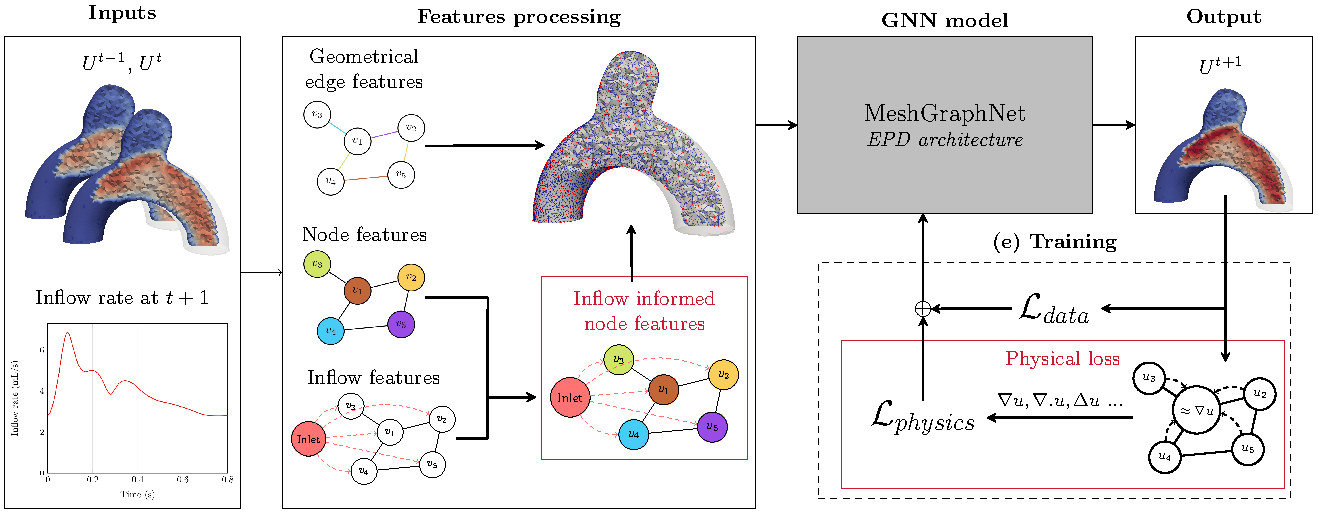
\includegraphics[width=1\textwidth]{figs/architecture.pdf}
    \caption{Model architecture - the input meshes and inflow data are exploited to create a feature graph, from which our GNN model can predict the next step mesh, taking into account physical and data losses combined during model training.}
    \label{fig:model}
\end{figure}


\subsection{Physically-constrained GNN} \label{sec:pinn}

Although the model is trained on datasets generated by an in-house numerical solver that computes solutions to the Navier-Stokes equations (see Subsection \nameref{sec:dataset}), the integration of physical knowledge into the training process can enhance the accuracy and reliability of its predictions. This approach aligns with the principles outlined in physics-informed machine learning, which has been shown to improve predictive performance by embedding domain-specific laws and constraints directly into the learning framework \cite{raissi_physics-informed_2019}.
 
 Moreover, data-only based learning approach can lack robustness to out-of-distribution cases. To enhance the performances of our model, we added a physics-based regularization through the addition of a more physically relevant loss (PI-GNN) by Suk et al. \cite{suk_physics-informed_2024}.
 
Thus, we approximated differentiable operators in a discrete vector field using gradient computation methods over unstructured graphs \todo{Reference to Methods}. 

\todo{Justify why finite difference, and maybe test with other approach to see if improvements}
% During this whole chapter, we used the finite-differences method for it's simplicity "and because there was no significant differences on the training results obtained when switching the gradient computation method. The  gradients were computed locally within each cell neighborhood on the mesh, to help preserve topological consistency even in geometrically complex zones."

From this gradient approximation, we could further compute approximations for the divergence $\nabla \cdot u_i$ used in the conservation of mass, as well as the convective term $u \cdot \nabla u$ and the viscous term $\mu \Delta u$. Using these approximations, we developed a physical loss function to augment our training by incorporating not only the discrepancies between predicted and ground truth velocities, but also a deeper understanding of the fundamental principles of fluid mechanics. This approach enables us to calculate a continuity loss based on the conservation of mass, as well as convective and viscous losses, which quantify the errors in the convective and viscous terms, respectively (\todo{ref to methods for NS}): 


\begin{align} \label{eq:loss_phy}
    \mathcal{L}_{continuity} &= \underset{v \in V}{\mathrm{mean}} \ \vert  (\nabla \cdot u)_v \vert \\
    \mathcal{L}_{convection} &= \underset{v \in V}{\mathrm{mean}} \ \vert \vert \rho u_v \nabla u_v - \rho \tilde{u_v} \nabla \tilde{u_v} \vert \vert^2_2 \\
    \mathcal{L}_{viscous} &= \underset{v \in V}{\mathrm{mean}} \ \vert \vert \mu \Delta u_v - \mu \Delta \tilde{u_v} \vert \vert^2_2
\end{align}

To mitigate the importance of each loss term during training, we combined the data and physical terms in a properly tuned weighted loss, as following: 

\begin{equation}
    \mathcal{L}_{PI} = \mathcal{L}_{data} + \alpha \mathcal{L}_{continuity} + \beta \mathcal{L}_{convection} + \gamma \mathcal{L}_{viscosity}
\end{equation}

with $\alpha$, $\beta$ and $\gamma$ being scaling factors. We tuned our weighted loss by evaluating the physical loss terms during the first epochs of training the data-only equivalent models, to adjust the scaling factors in order to get comparable scales for each contributor of the global loss. The data loss term was given a weight of 0.5, while the remaining physics-informed terms were equally distributed over the remaining 0.5. While the continuity term stabilizes after only one epoch, the convection and viscosity losses decrease steadily during the whole training along side with the data loss, providing a faster model convergence.

\todo{talk about the residual stuff with CFD: trying to learn 2 things at once}

\subsection{Evaluation metrics}

To compare the performances of our models, we computed the L2 norm of the velocity error, and with this error the Root Mean Square Error (RMSE) averaged across case geometry. We used the 1-RMSE to evaluate the next-step predictions of our model, as well as the 50-RMSE on a rollout prediction to determine the robustness of the model on full trajectory predictions, as formulated in \autoref{eq:rmse}. We displayed these errors, averaged on the test set, in \autoref{tab:model-configurations} \todo{missing ref}, as well as the standard deviation of the 50-step RMSE to evaluate the stability of the models on different test cases. These errors are in mm/s, and the values reported in \autoref{tab:model-configurations} are absolute errors, not normalized by maximum velocity.

\begin{equation}\label{eq:rmse} 
\begin{split}
    1\textrm{-RMSE} &= \sqrt{\frac{\sum_i^N (y_i^t - f(x^{t-1})_i)^2}{N}}\\
    T\textrm{-RMSE} &= \frac{1}{T}\sum_t^T \sqrt{ \frac{\sum_i^N (y_i^t - f^t(x^0)_i)^2}{N} }
\end{split}
\end{equation}

Three representative cases were randomly chosen from the 10 test cases while guaranteeing coverage of three bulge sizes. Three key timesteps were also selected along the cardiac cycle as shown in  \autoref{fig:eval_cases} \todo{MISSING REG}, to represent the systolic, peak systole and diastolic phases. We computed WSS as well as time-averaged WSS (TAWSS) as defined in \nameref{sec:Methods} \todo{MISSING REG} to further analyze the predictions capability of the models needed for risk assessment. All WSS-based quantities were derived directly from the velocity fields, and were not interpolated from the finer cases. We also plotted the aneurysm neck plane to show the velocity of the flow entering and exiting the bulge, as well as on three selected points along the full cardiac cycle to show the velocity evolution inside the neck, the outflow artery and close to the bulge wall, as shown in \autoref{fig:eval_cases}. The mentioned velocity and WSS errors are normalized by the ground truth maximum at a given timestep; because of the highly dynamic nature of the flow, normalizing by the overall maximum value would highly reduce the error on every timestep far from the peak systole.
